\documentclass[twoside]{amsart}
\usepackage{amsmath,amsthm,amsfonts,amssymb}
\usepackage{color}
\usepackage[pagebackref,colorlinks,citecolor=blue,linkcolor=blue,urlcolor=blue,filecolor=blue]{hyperref}
\usepackage{tikz}
\usetikzlibrary{shapes.geometric}
\tikzset{
v/.style={draw, fill, circle, minimum size=1.5mm, inner sep=0},
b/.style={draw , regular polygon,regular polygon sides=4, minimum size=1.5mm, inner sep=.5mm},
e/.style={very thick},
vs/.style={draw, fill, circle, minimum size=1mm, inner sep=0},
bs/.style={draw,  regular polygon,regular polygon sides=4, minimum size=2mm, inner sep=0mm},
es/.style={thick}
}
\usetikzlibrary{arrows,matrix,positioning}

\begin{document}

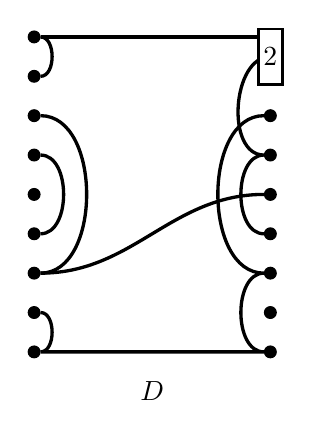
\begin{tikzpicture}[x=1.5cm,y=-.5cm,baseline=-2.05cm]
    
        \node[v] (a1) at (0,0) {};
        \node[v] (a2) at (0,1) {};
        \node[v] (a3) at (0,2) {};
        \node[v] (a4) at (0,3) {};
        \node[v] (a5) at (0,4) {};
        \node[v] (a6) at (0,5) {};
        \node[v] (a7) at (0,6) {};
        \node[v] (a8) at (0,7) {};
        \node[v] (a9) at (0,8) {};
        
        \node[v] (b3) at (2,2) {};
        \node[v] (b4) at (2,3) {};
        \node[v] (b5) at (2,4) {};
        \node[v] (b6) at (2,5) {};
        \node[v] (b7) at (2,6) {};
        \node[v] (b8) at (2,7) {};
        \node[v] (b9) at (2,8) {};

        
        \draw[e] (a1) to[out=0, in=180] (2,0);      
        \draw[e] (a7) to[out=0, in=180] (b5);
        \draw[e] (a1) to[out=0, in=0] (a2);
        \draw[e] (a8) to[out=0, in=0] (a9) to[out=0, in=180] (b9) to[out=180, in=180] (b7) to[out=180, in=180] (b3);
        \draw[e] (a3) to[out=0, in=0]   (a7);
        \draw[e] (a4) to[out=0, in=0]   (a6);
        \draw[e] (2,0.5) to[out=180, in=180](b4) to[out=180, in=180] (b6);
        \draw[fill=white, line width=1] (1.9,-0.2) rectangle (2.1,1.2);
        \node at (2,0.5) {$2$};
        \node at (1,9) {$D$};
    \end{tikzpicture}

\end{document}